The inclusive \wh{} fit follows the STXS binning strategy to keep consistency across analyses. The only distinction between the inclusive and STXS fits lies in the number of parameters of interest (POIs). In the inclusive case, a single POI is used for the signal strength in each individual channel as well as for the combination of the \zdom{} and \zdep{} channels.

From the fit, the expected signal strengths in the \zdom{}, \zdep{}, and combined channels are found to be $\mu = 1.02^{+0.71}_{-0.66}$, $\mu = 1.01^{+0.57}_{-0.49}$, and $\mu = 1.00^{+0.43}_{-0.39}$, respectively. The corresponding observed results are $\mu = 0.40^{+0.81}_{-0.75}$, $\mu = 1.16^{+0.59}_{-0.49}$, and $\mu = 0.82^{+0.45}_{-0.39}$. A profile likelihood scan of both the expected and observed signal strengths is shown in Figure~\ref{fig:wh_3l_inclusive_likelihood_scan}.

\begin{figure}[htp]
  \centering
  \subfloat[Expected likelihood scan.]{
    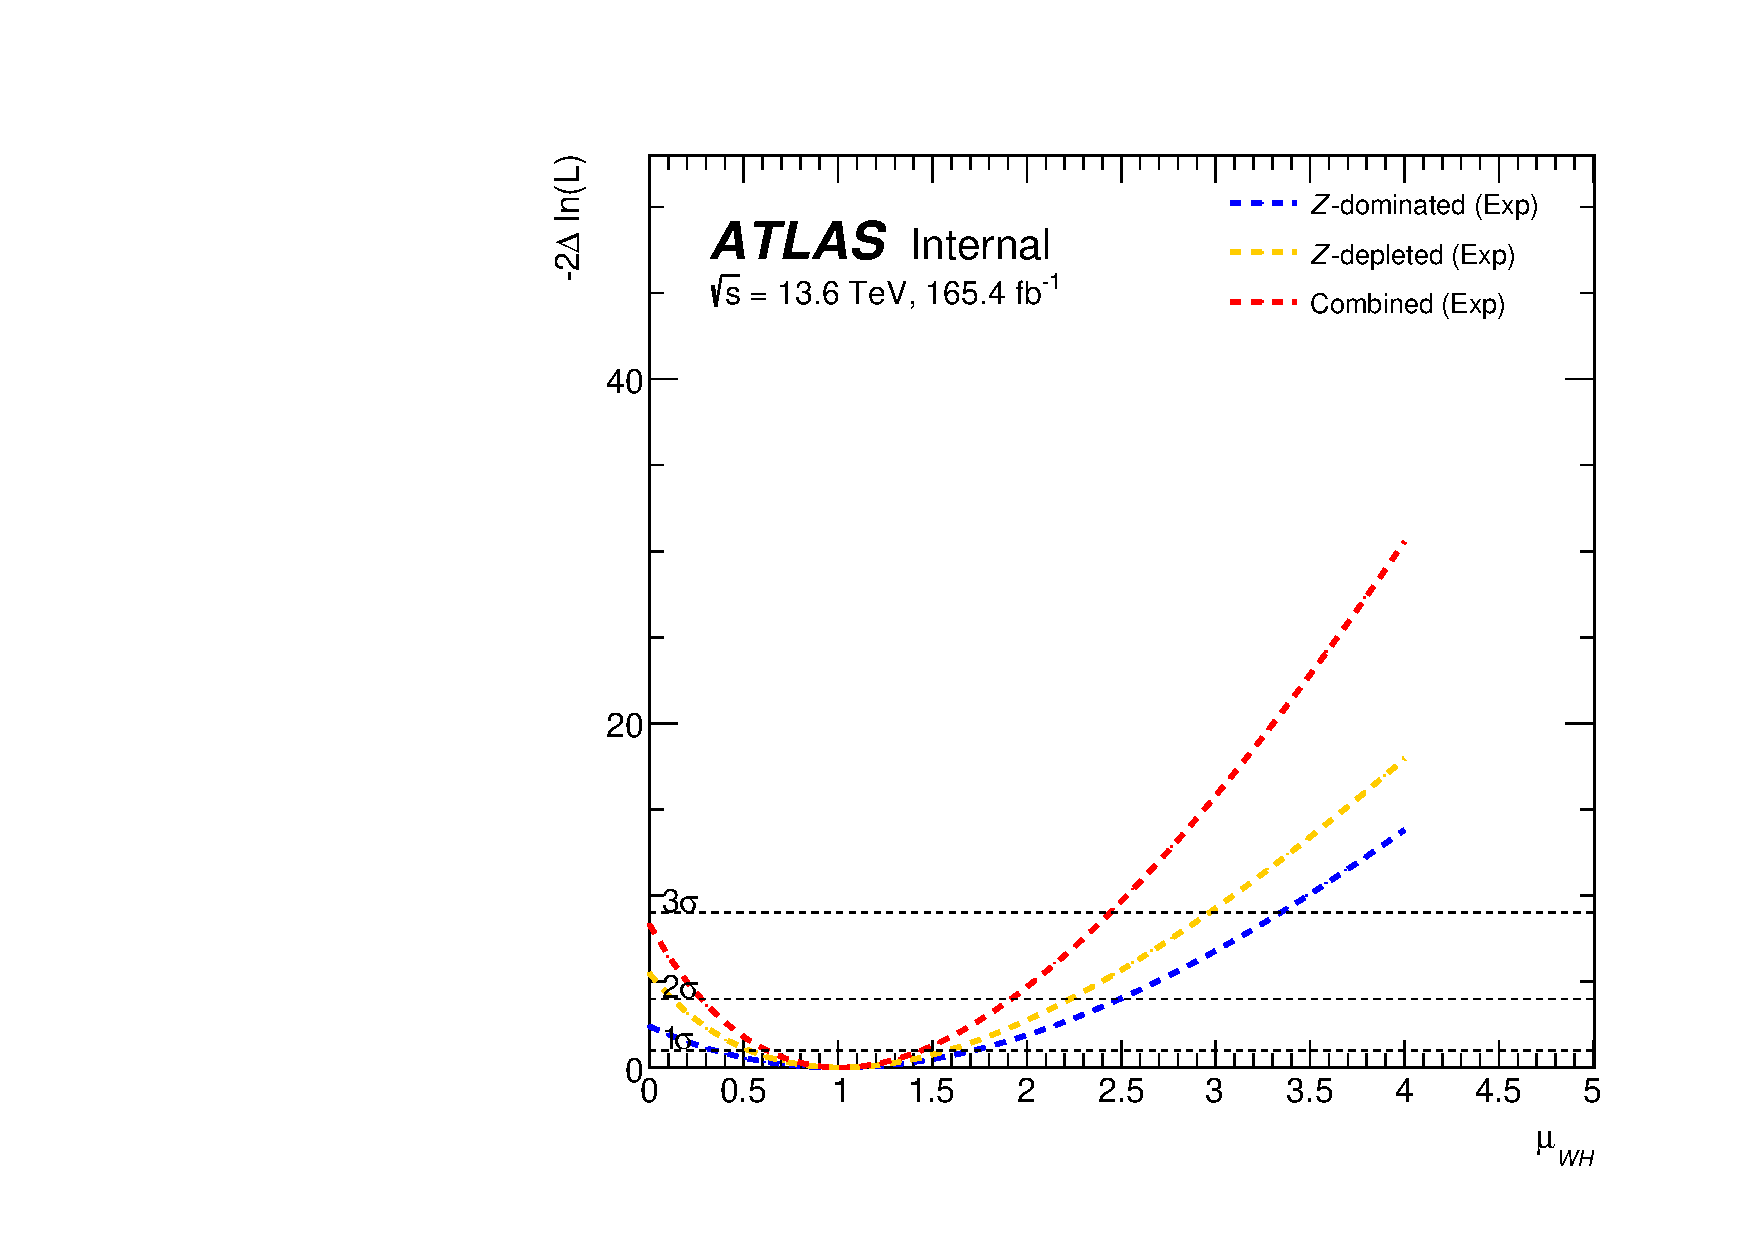
\includegraphics[width=0.48\linewidth]{figures/statistical/nll_plots_wh_expected.pdf}
  }
  \subfloat[Observed likelihood scan.]{
    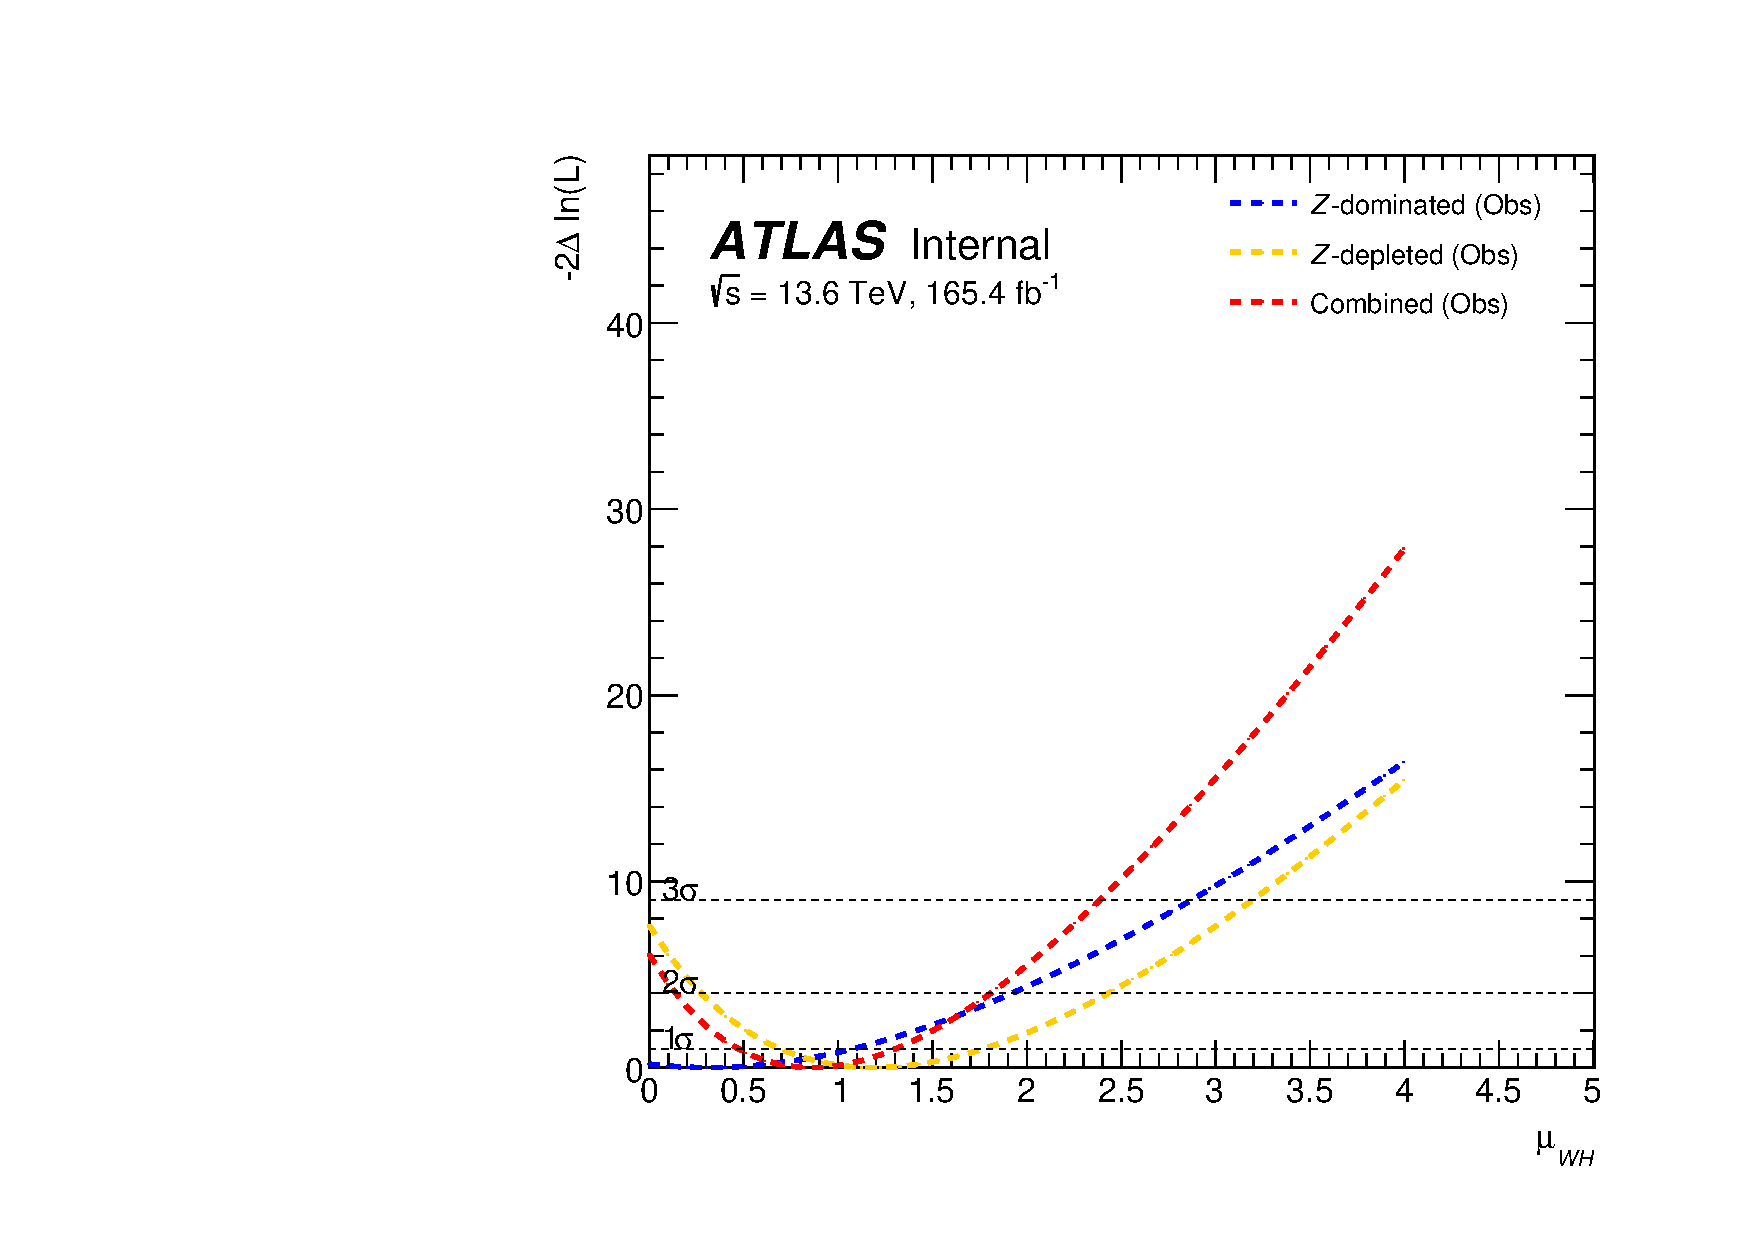
\includegraphics[width=0.48\linewidth]{figures/statistical/nll_plots_wh_observed.pdf}
  }
  \caption{Likelihood scans for the three \wh{} signal regions: (a) expected and (b) observed.}\label{fig:wh_3l_inclusive_likelihood_scan}
\end{figure}


To study the impact of statistical and systematic uncertainties on the \wh{} measurement, we present the pulls in Appendix~\ref{app:wh_pull_plots}, the correlations between uncertainties in Appendix~\ref{app:wh_correlation_plots}, and the systematic ranking plots in Appendix~\ref{app:wh_ranking_plots}.
The most relevant post-fit distributions for the \wh{} SRs are shown in Figures~\ref{fig:wh_3l_postfit_zdom}.

\begin{figure}[htp]
  \centering
  \subfloat[$\ensuremath{\ptw \in \left[0,75\right)}$~GeV.]{
    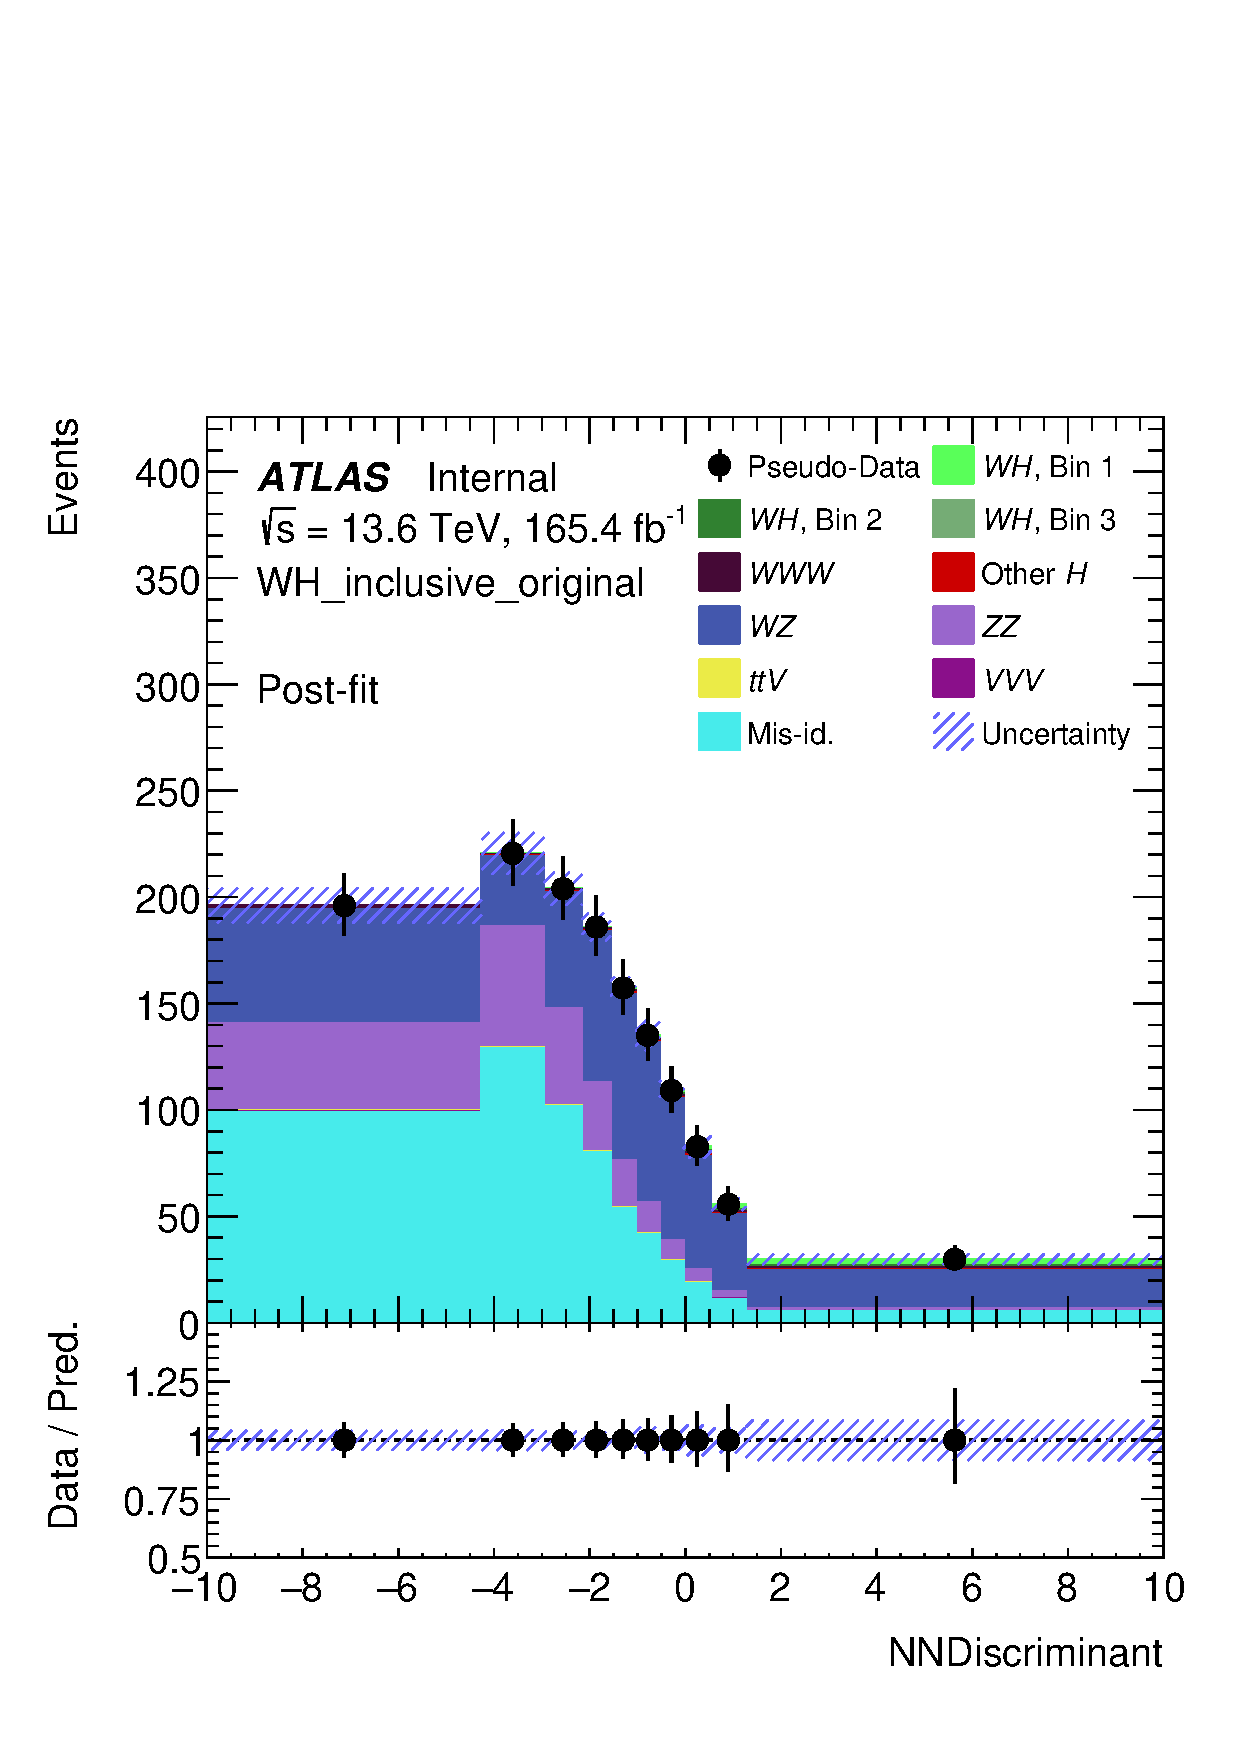
\includegraphics[width=0.29\linewidth]{figures/statistical/NNDiscriminant_zdom_0to75_postFit.pdf}
  }
  \subfloat[$\ensuremath{\ptw \in \left[75,150\right)}$~GeV.]{
    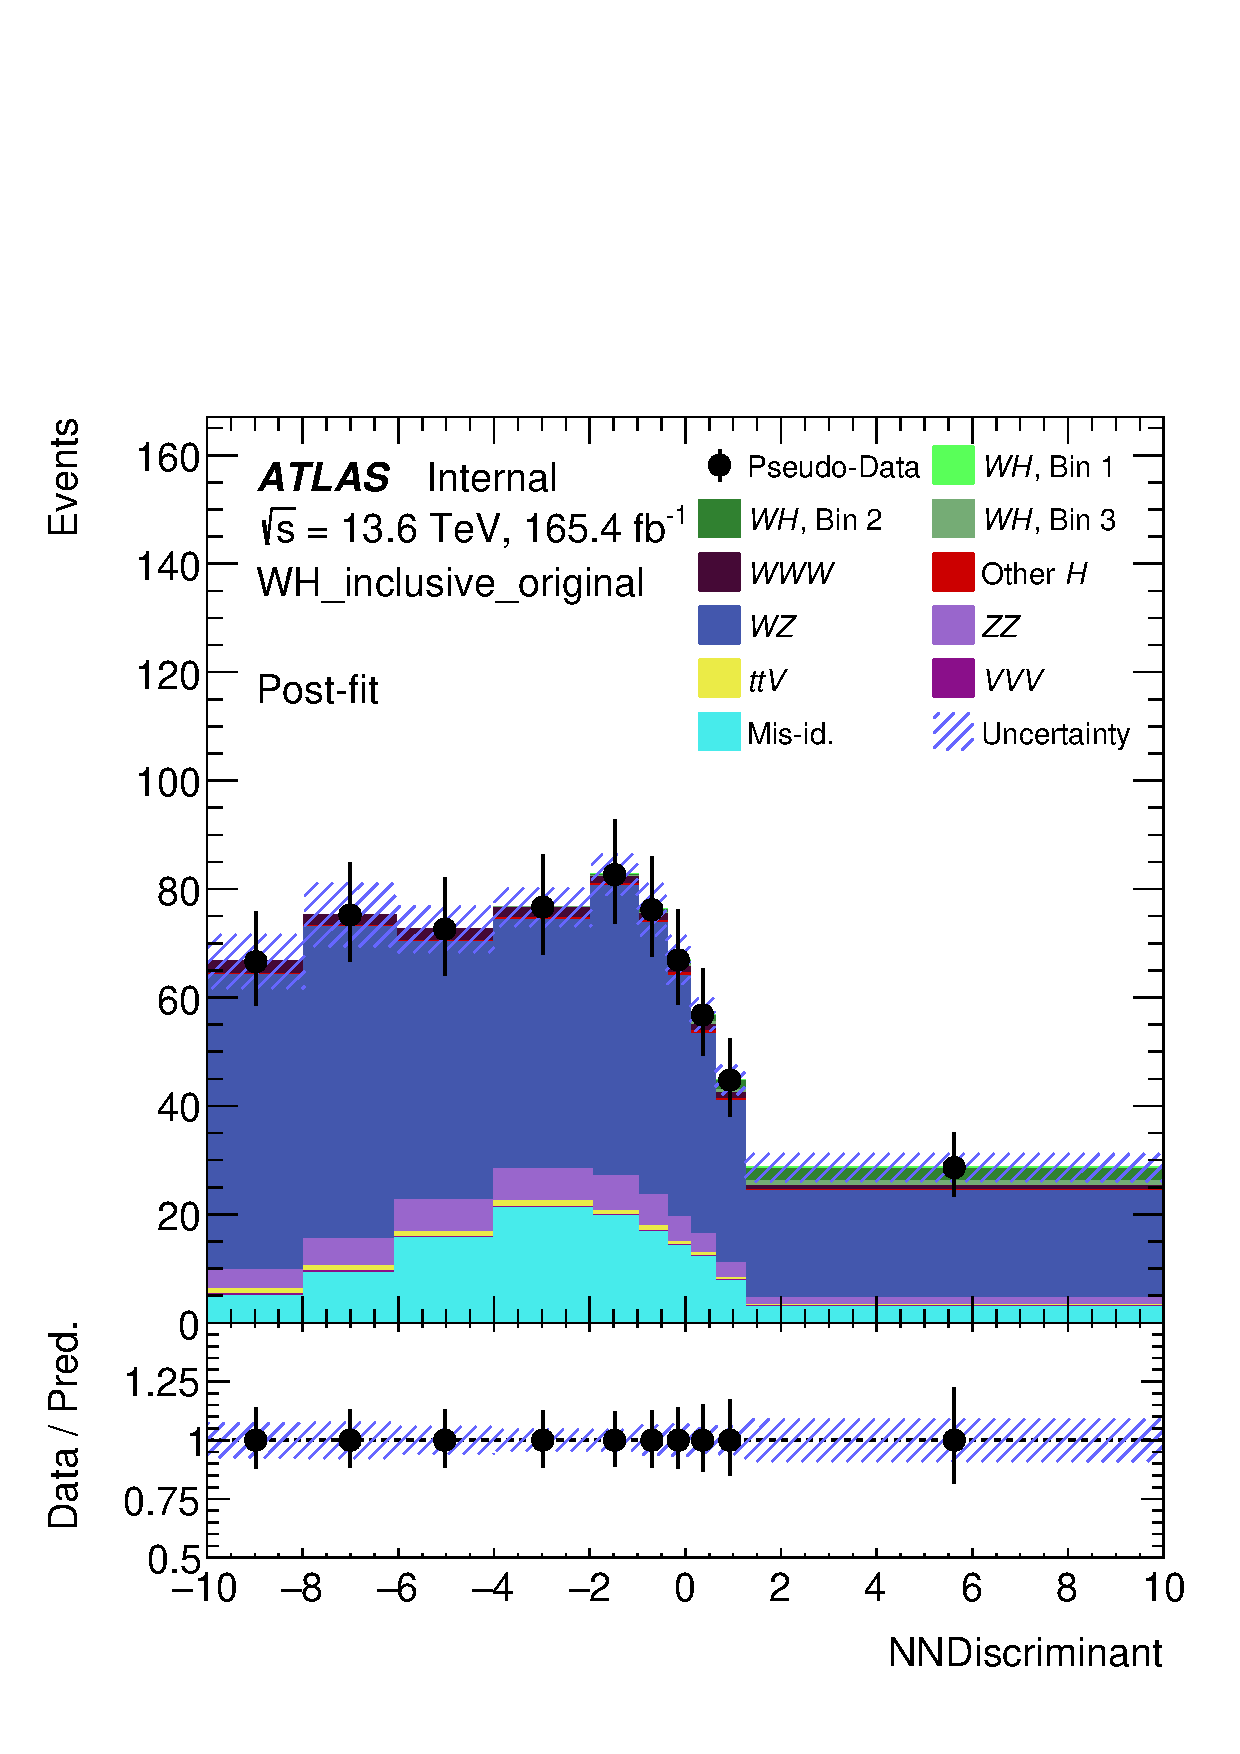
\includegraphics[width=0.29\linewidth]{figures/statistical/NNDiscriminant_zdom_75to150_postFit.pdf}
  }
  \subfloat[$\ptw \geq 150$~GeV.]{
    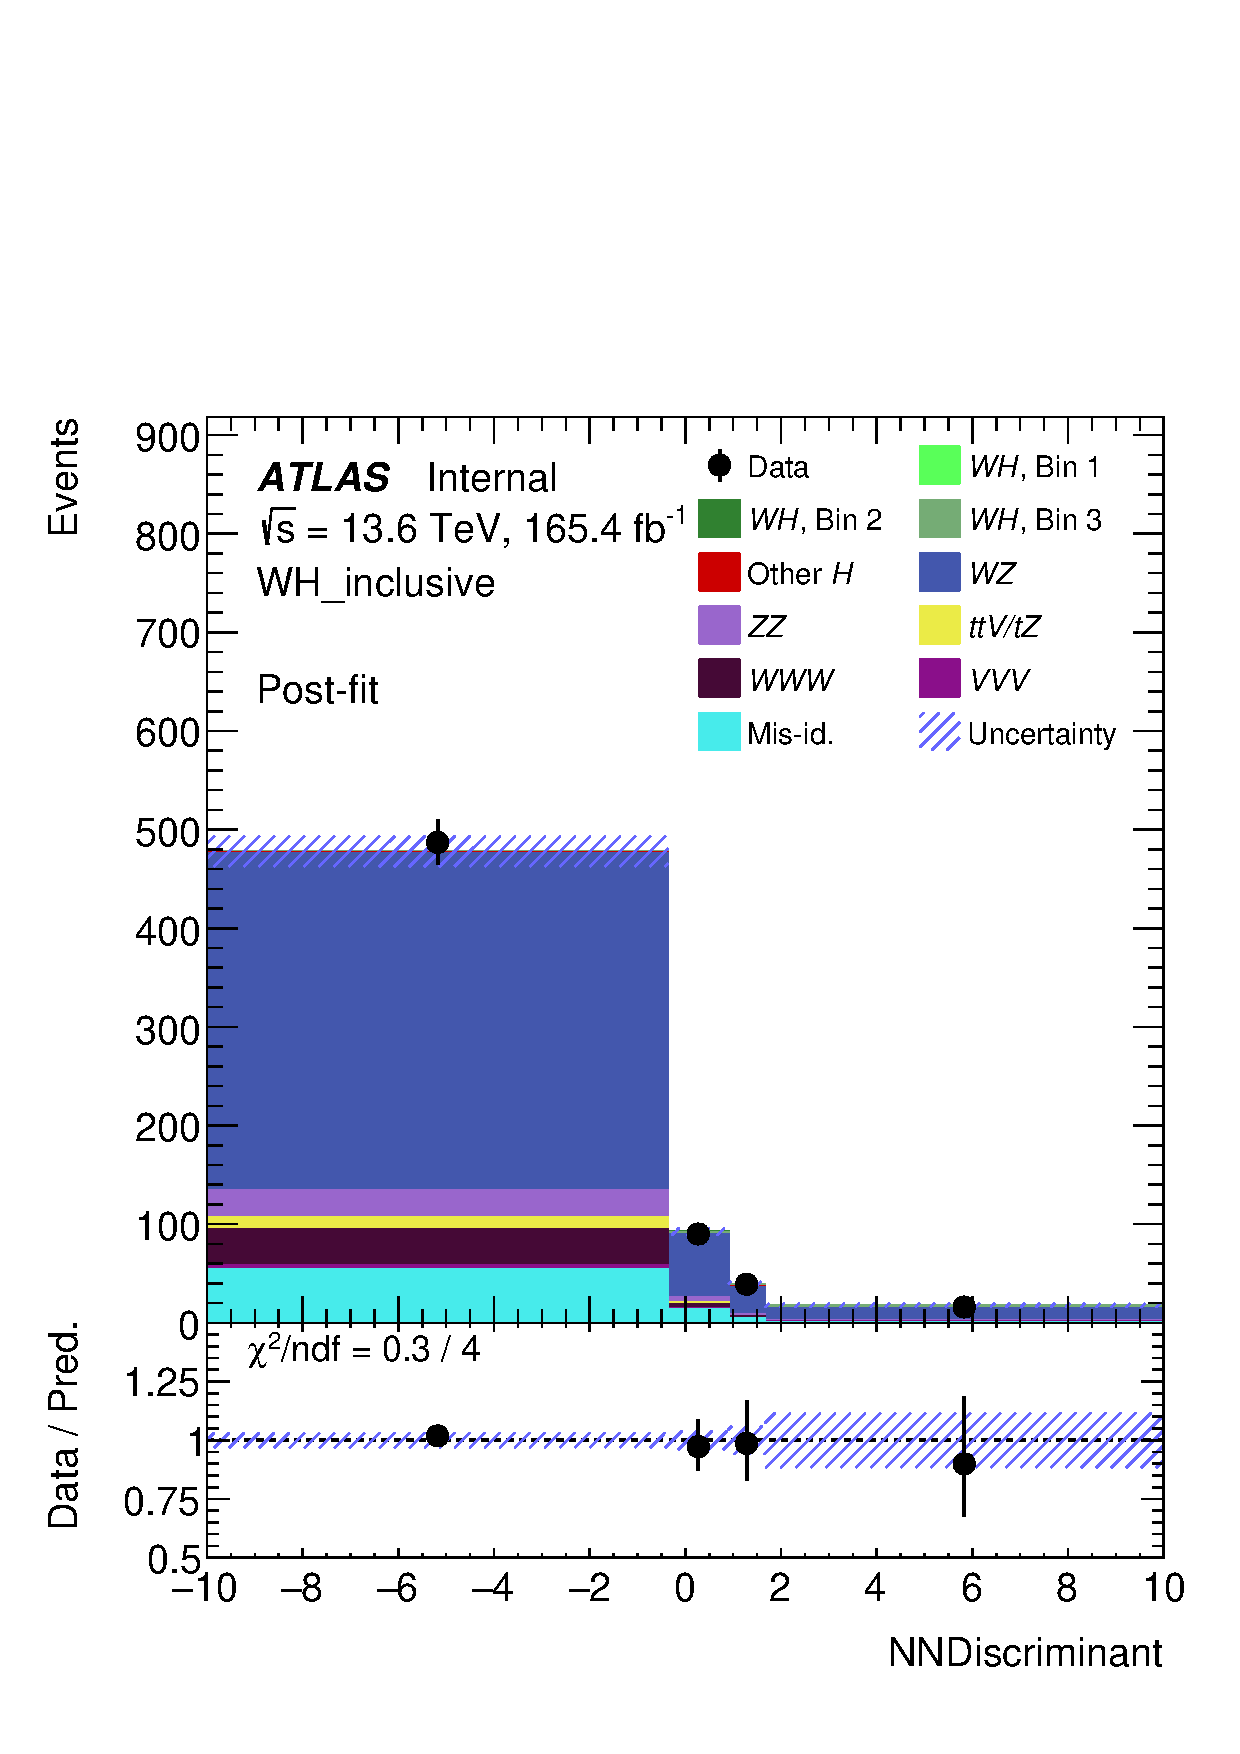
\includegraphics[width=0.29\linewidth]{figures/statistical/NNDiscriminant_zdom_150toinf_postFit.pdf}
  } \\
  \subfloat[$\ensuremath{\ptw \in \left[0,75\right)}$~GeV.]{
    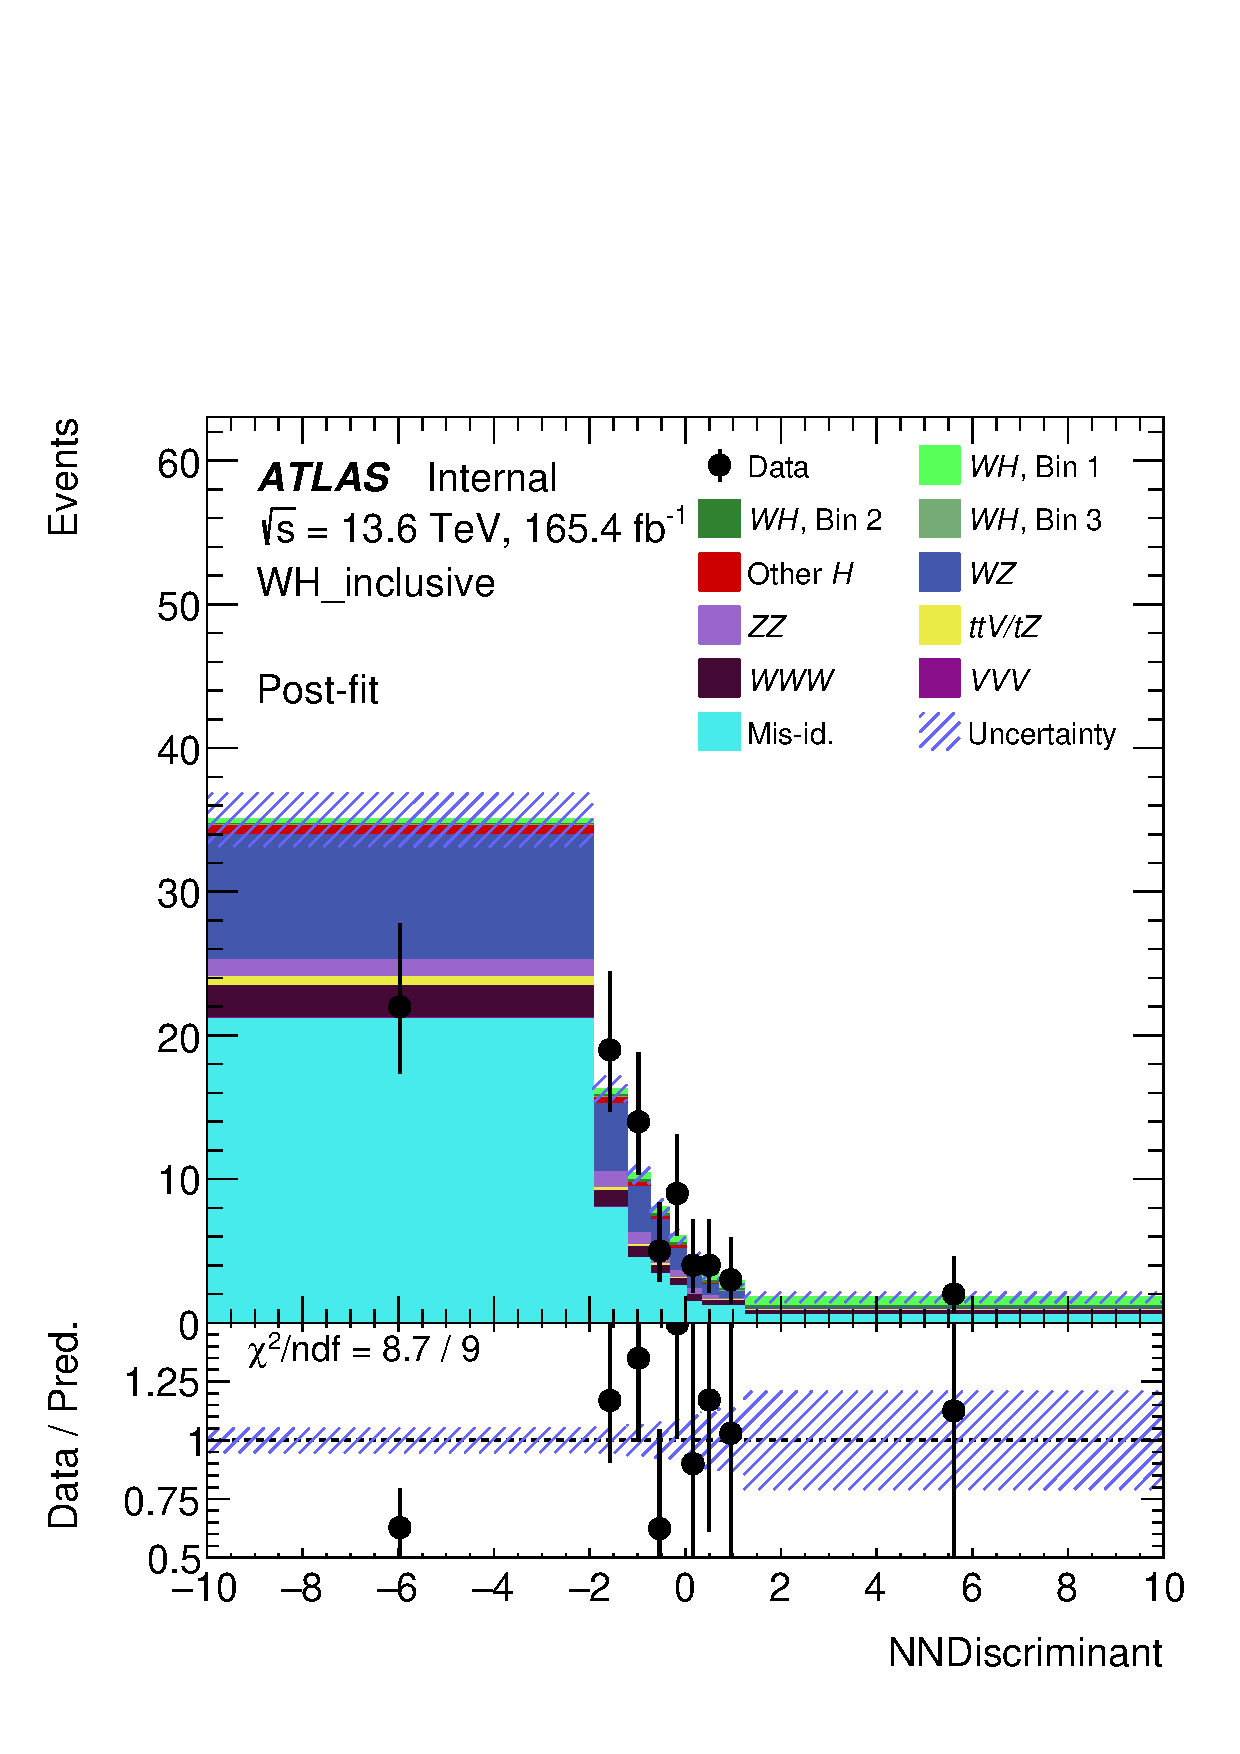
\includegraphics[width=0.29\linewidth]{figures/statistical/NNDiscriminant_zdep_0to75_postFit.pdf}
  }
  \subfloat[$\ensuremath{\ptw \in \left[75,150\right)}$~GeV.]{
    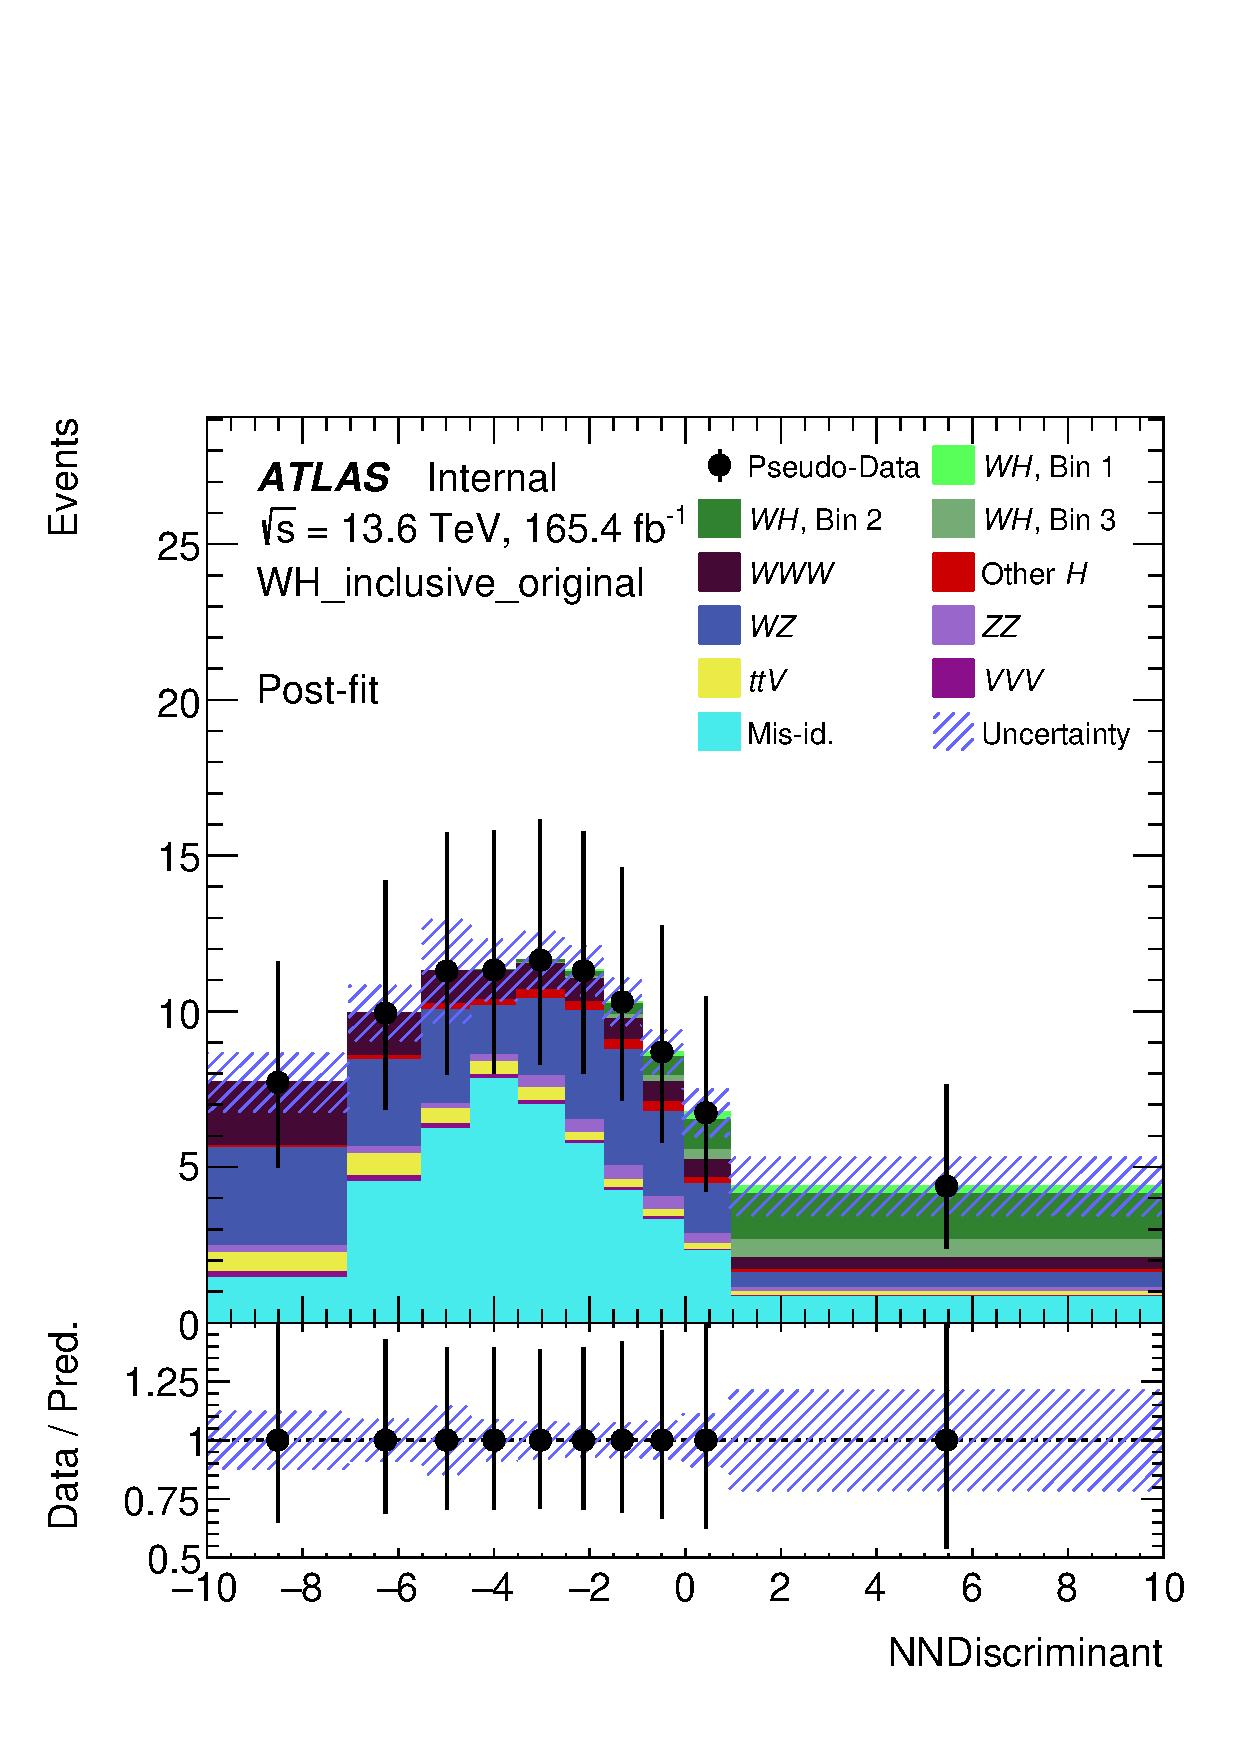
\includegraphics[width=0.29\linewidth]{figures/statistical/NNDiscriminant_zdep_75to150_postFit.pdf}
  }
  \subfloat[$\ptw \geq 150$~GeV.]{
    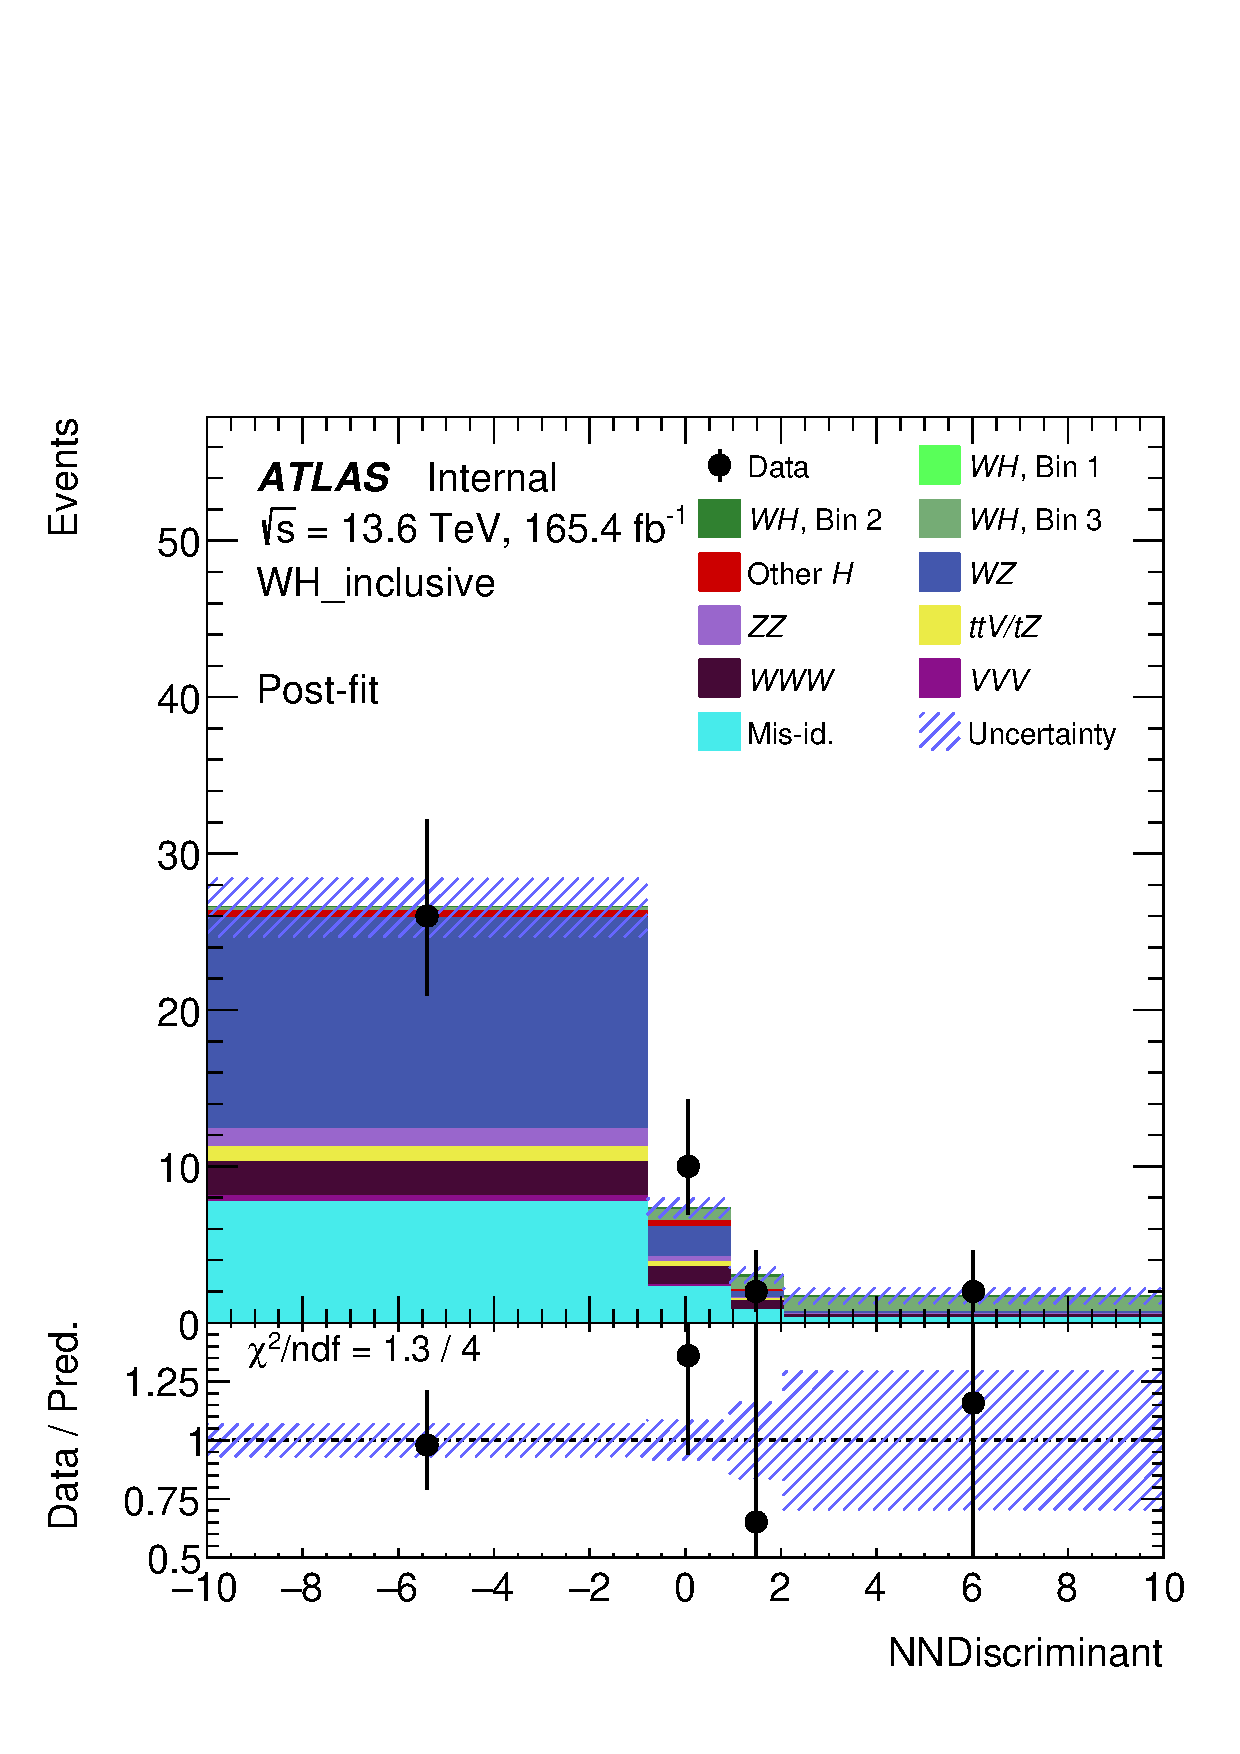
\includegraphics[width=0.29\linewidth]{figures/statistical/NNDiscriminant_zdep_150toinf_postFit.pdf}
  }
  \caption{Post-fit NN discriminant distributions in the signal regions: 
  \zdom{} in the top row and \zdep{} in the bottom row.
  Columns correspond to STXS bins defined by $\ptv$: 
  (a,d) 0--75~GeV, (b,e) 75--150~GeV, (c,f) $\geq$150~GeV.}\label{fig:wh_3l_postfit_zdom}
\end{figure}

The NFs for the $WZ$ CR's are found to be $\text{NF}_{WZ~\text{0 Jets}} = 0.91^{+0.10}_{-0.10}$, $\text{NF}_{WZ~\text{1 Jet}} = 0.92^{+0.12}_{-0.12}$, and $\text{NF}_{WZ~\text{2+ Jets}} = 0.87^{+0.16}_{-0.16}$. The NF for the $WWW$ CR is found to be $\text{NF}_{WWW~\mathrm{CR}} = 1.84^{+0.71}_{-0.66}$. This $WWW$ NF is consistent with those found in the previous Run~2 $VH$ analysis, as well as the measurement of the measurement of the $WWW$ cross section. 

\noindent{} All results from the \wh{} channel are summarized in Tables~\ref{tab:wh_inclusive_results_summary}.

\begin{table}
  \centering
  \begin{tabular}{l|c|c|c}
    \hline
    \multicolumn{4}{c}{\textbf{Results Summary}}\\
    \hline
     & \zdom{} SR & \zdep{} SR & \wh{} channel\\
    \hline
    $\mu_{WH}$ (Expected) & $1.01^{+0.71}_{-0.66}$ & $1.01^{+0.57}_{-0.49}$ & $1.01^{+0.43}_{-0.39}$ \\
    $\mu_{WH}$ (Observed) & $0.40^{+0.81}_{-0.75}$ & $1.16^{+0.59}_{-0.49}$ & $0.82^{+0.45}_{-0.39}$ \\
    NF $WZ$ 0 Jets & $0.94^{+0.07}_{-0.07}$ & $0.93^{+0.07}_{-0.07}$ & $0.91^{+0.10}_{-0.10}$ \\
    NF $WZ$ 1 Jet & $0.93^{+0.08}_{-0.08}$ & $0.92^{+0.08}_{-0.08}$ & $0.92^{+0.12}_{-0.12}$ \\
    NF $WZ$ 2+ Jets & $0.90^{+0.13}_{-0.13}$ & $0.89^{+0.13}_{-0.13}$ & $0.87^{+0.16}_{-0.16}$ \\
    NF $WWW$ VR & N/A & $1.58^{+0.61}_{-0.56}$ & $1.84^{+0.71}_{-0.66}$ \\
    \hline
    Significance (Expected) & $1.3\sigma$ & $2.4\sigma$ & $2.7\sigma$ \\
    Significance (Observed) & $0.5\sigma$ & $2.7\sigma$ & $2.3\sigma$ \\
    \hline
  \end{tabular}
  \caption{Summary of the expected and observed signal strengths, NFs, and significances for the \wh{} inclusive fit, broken down into individual channels as well as the combined results.}\label{tab:wh_inclusive_results_summary}
\end{table}